\chapter{Theory Introduction}  % should probably change this name
\label{theory}

\section{The Standard Model}
\label{theory:SM}

% http://www.symmetrymagazine.org/cms/?pid=1000064  the symmetry magazine SM picture
% don't know how it prints in black and white
% LATEX DOESN'T DO GIFS

 \begin{figure}[htb]
  \begin{center}
    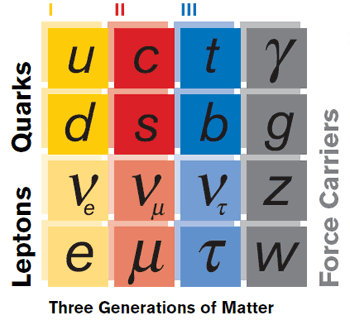
\includegraphics[width=360pt]{Figures/theory-standard-model-symmetry-mag.png}
  \end{center}
  \caption[Particles of the standard model]
	  {Particles of the standard model that are known to exist. 
	    The Higgs boson is also predicted as part of the 
	    Standard Model, 
	    but has not yet been discovered. 
	    }
  \label{fig:StandardModel}
 \end{figure}


quarks, leptons, bosons!  HIGGS ha ha

gauge groups, little intro to group theory

put all qcd stuff in here?  don't need all the detail of zeus stuff

\section{Electroweak Physics}
\label{theory:EWK}

lagrangian etc? i.e. more specifics on ewk physics

feynman diagrams, how they can actually be used -> 
matrix elements -> cross section element.  

where to put cross section formula stuff 
-- make new section?
(and which stuff to use?)

order of diagram = number of vertices!  

\subsection{Z Production}
\label{theory:Zprod}

previous results here?

\subsection{Z Decay}
\label{theory:Zdec}
need this section??


somewhere have intro to QFT and all that?  

also, explanatory items from overview:

   * [here or] in theory chapter define ``tree-level''.  
ALSO IN THEORY: explain how Feynman diagrams are so useful! 
writing down the matrix element and all that
AND PDFs, basically whole process of stuff simulated 
really happens and should be explained.  
AND DEF OF PARTONS
yeah, basically explain all the stuff in the MC chapter
INCLUDING ISR and FSR
ALSO define ``jets'' and talk about how they come from 
quarks and gluons (define partons) and relate to ``hadronization'' -- 
not entirely relevant for this analysis, 
but possible in general
AND define ``color''
AND asymptotic freedom, how it takes more and more energy to get them further apart

   * intial- and final-state radiation

   * [HERE OR IN THEORY INTRO] need to do on-shell/off-shell decays 
to explain why Z mass has a spectrum and not a single value

   * invariant mass (here?)

   * cross section formula and matrix elements and what said matrices do

AND, of course read the others' theses to see what they had in here, too.  



